\graphicspath{{\relativepath/figures/}}

\section{Global presentation of the components of the simulator}
\label{sec:global}

\subsection{Components of the simulator}

\begin{figure}[!ht]
        \centering
        \includegraphics[width=\linewidth]{presentation}
	\caption{Schematical view of the simulator.}
\label{fig:presentation}
\end{figure}

The simulator can be decomposed into several large modules
that handle specific tasks during simulation~\reffigp{fig:presentation}.
First of all, there is an \textbf{input/output} module that creates everything
that is needed for the simulation from an input file.
\textbf{Reactants} and \textbf{reactions} are user-specified and need to be created on demand,
as well as \textbf{events} happening throughout the simulations
and more technical aspects about which algorithm to use to perform the integration.
Once everything is set up, the \textbf{solver} follows a simple loop
that can be decomposed in three steps.
Integration occurs reaction by reaction, at each loop, we go forward one reaction,
update the simulation time, concentrations and reaction rates.

\begin{enumerate}
	\item At the beginning of the loop,
  the \textbf{input/output} process checks whether \textbf{events}
  should occur at the current simulation time and
  whether it needs to write some concentrations to an output file.
	\item It then hands control over to the \textbf{solver},
  which is based on Gillespie's approach to integrate a network of chemical reactions.
  The Gillespie algorithm needs the current reaction rates of all \textbf{reactions}
  and draws a random reaction with a probability proportional to its rate.
  This task is delegated to a \textbf{rate manager},
  which uses state-of-the-art methods to maintain the rate list updated and perform the drawing efficiently.
	\item Once a \textbf{reaction} is drawn, it is performed.
  The concentrations (and the state, see below) of its \textbf{reactants} are modified.
\end{enumerate}


% subsection presenting reactant classes

\subsection{Reactants}

\subsubsection{\texttt{FreeChemical}}

\texttt{FreeChemical} simply represents a pool of interchangeable molecules distributed uniformly in the cell.
Computationally, only the number of molecules in the pool is relevant.

\subsubsection{\texttt{BoundChemical}}

\begin{figure}[!h]
  \centering
  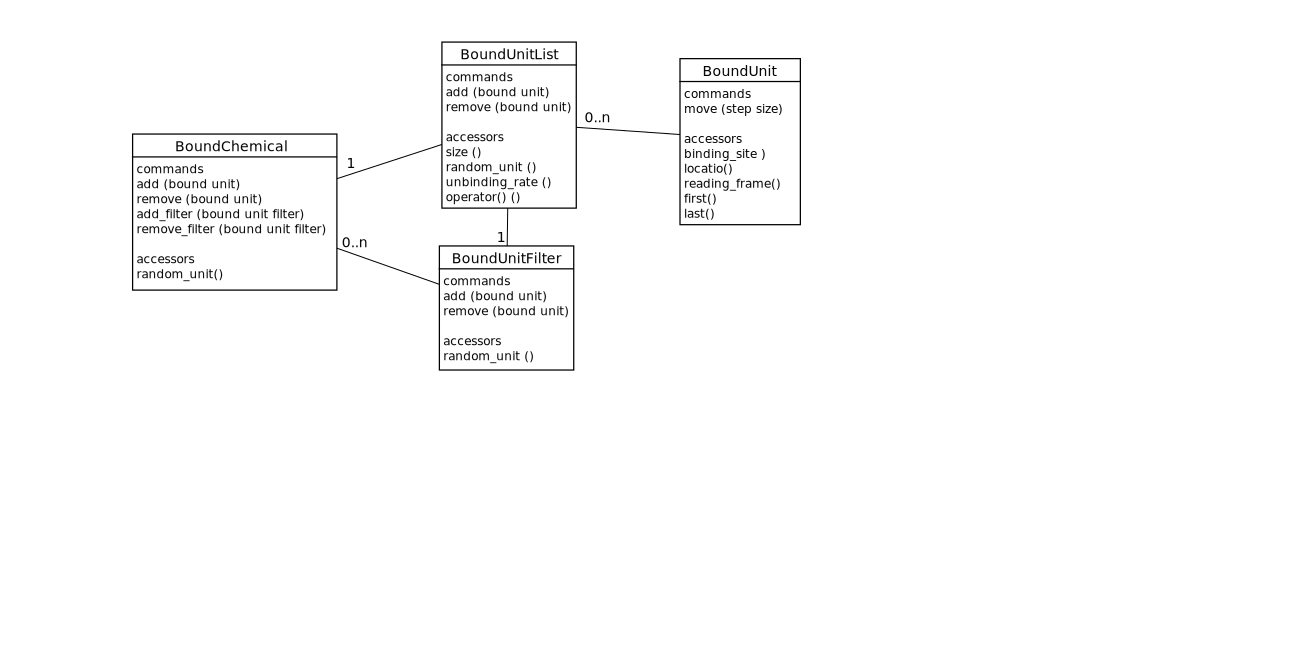
\includegraphics[width=\linewidth]{boundchemical}
  \caption{
  \texttt{BoundChemical} are in fact a pool of individual \texttt{BoundUnit}
  created using a \texttt{BoundUnitFactory}.
  A \texttt{BoundUnit} is characterized by the \texttt{ChemicalSequence}
  it bound to and its current position.
  Reaction then use \texttt{BoundUnitFilter} to sort \texttt{BoundUnit}
  according to some criterium of reference
  (\textit{e.g.} \texttt{Loading} reactions sort \texttt{BoundUnit} according to the motif they read).
  }
\label{fig:det_bound_chemical}
\end{figure}

\texttt{BoundChemical} represents molecules of the same chemical species,
but there are specificities for each unit of a \texttt{BoundChemical},
as all units are bound at different locations of different
\texttt{ChemicalSequence}~\reffigp{fig:det_bound_chemical}.
A \texttt{BoundUnitFactory} is used to recycle \texttt{BoundUnit}s,
avoiding memory reallocation throughout simulation.
\texttt{BoundUnitFilters} are used to sort \texttt{BoundUnit}s according
to criteria useful for reactions~\reffigp{fig:det_bound_chemical}.

\texttt{BoundUnit}s are passed from one \texttt{BoundChemical} species to another through reactions,
their attributes are updated if needed.
They are only destroyed once they are unbound from their \texttt{ChemicalSequence}.


\subsubsection{\texttt{ChemicalSequence}}

\begin{figure}[!h]
  \centering
  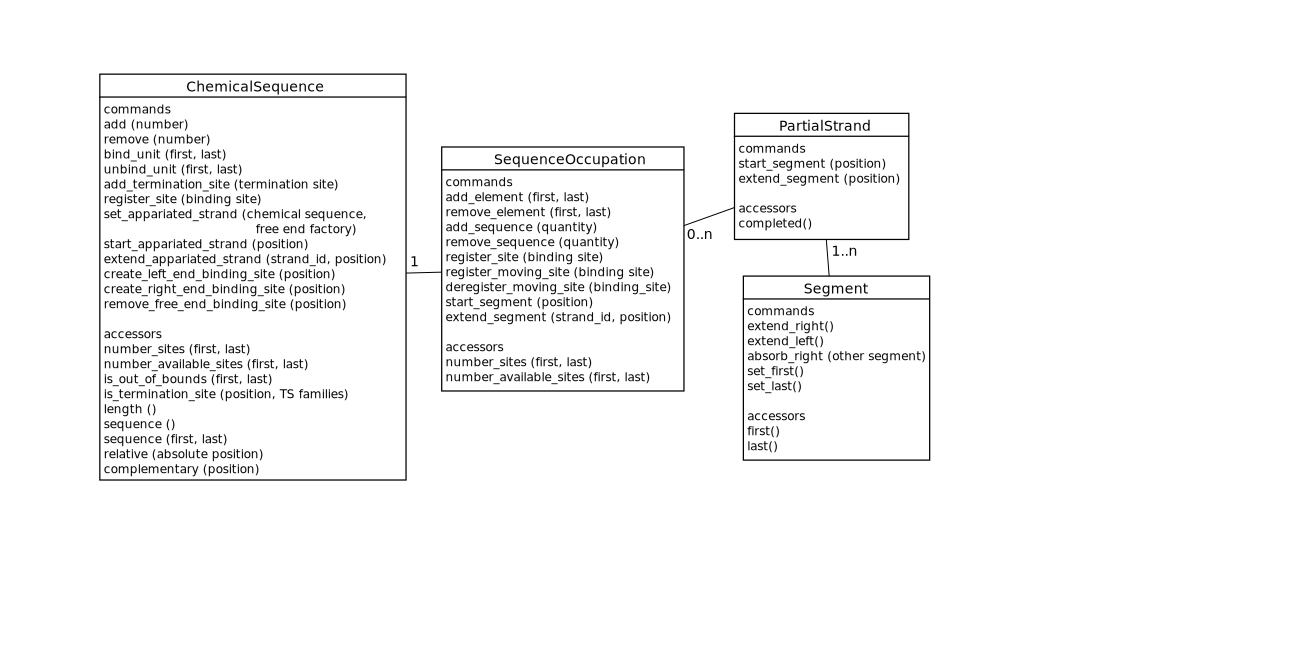
\includegraphics[width=\linewidth]{chemicalsequence}
  \caption{
  \texttt{ChemicalSequence} represents a pool of polymers that can be elongated
  and on which \texttt{BoundUnit}s bind through \texttt{BindingSite}s.
  For binding to occur, availability of \texttt{BindingSite} is assessed
  using a utility class \texttt{SequenceOccupation}
  that records the number of instances of the polymer,
  the position of \texttt{BoundUnit}s and elongation of \texttt{PartialStrand}s.
  \texttt{SiteGroup} is used to notify sites of availability changes more efficiently.}
\label{fig:det_chemical_sequence}
\end{figure}

\texttt{ChemicalSequence} handles a pool of polymers.
A pool is defined by a \emph{master sequence} describing what a typical polymer
looks like (\textit{e.g.} the sequence of DnaA protein)
and the number of \emph{instances} of the master sequence in the pool.
For efficiency reason, we do the following assumptions.

\paragraph{Simplifying assumptions}
\begin{itemize}
\item No deviation from master sequence, all instances are identical.
\item \texttt{BoundUnit}s are not assigned to a specific instance of the sequence,
they are positioned on the  master sequence.
\end{itemize}

\subparagraph{Consequences}
\begin{itemize}
\item No direct inference of collisions is possible.
\item A chemical can bind on a partial strand, yet move along the whole sequence freely.
\item Degradation of an instance does not cause unbinding.
\end{itemize}

\paragraph{Site availability}
Despite our simplifying assumptions it is still possible to provide
an accurate description of site availability.
Availability depends of the number of sequences, number and position of bound elements,
number and position of newly polymerized sequence segments~\reffigp{fig:det_chemical_sequence}.


\subsubsection{\texttt{DoubleStrand}}

\begin{figure}[!h]
  \centering
  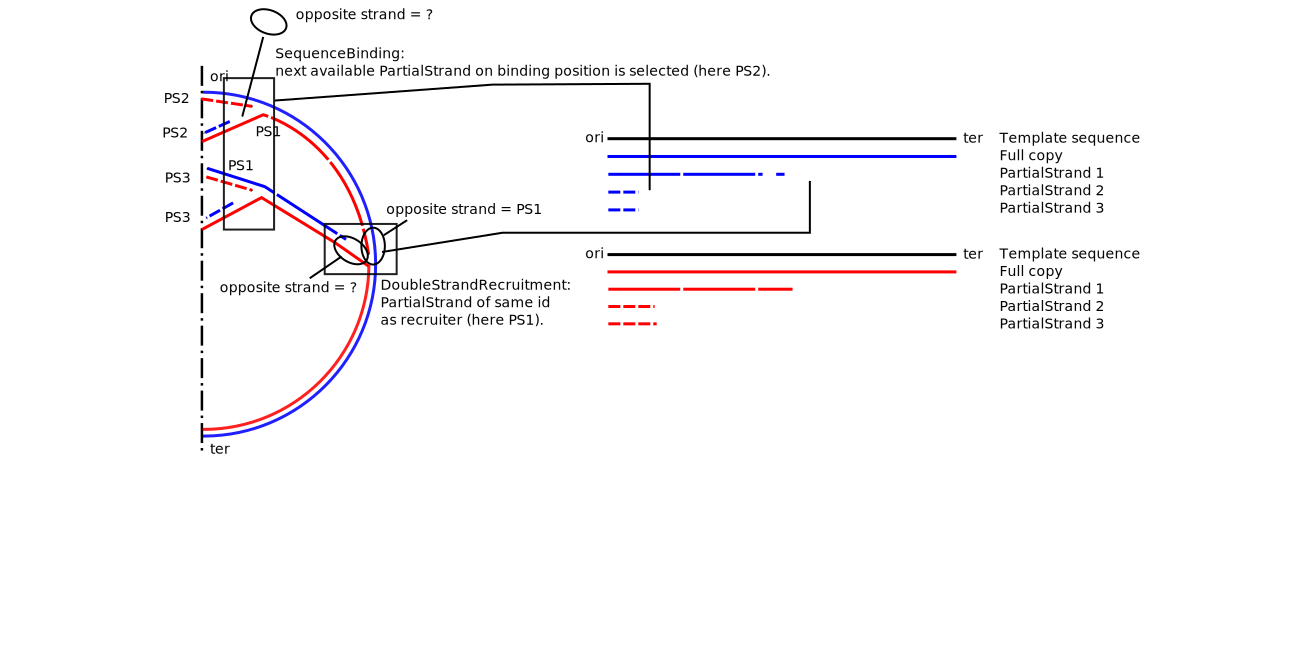
\includegraphics[width=\linewidth]{strand_id}
  \caption{
  Strands of a \texttt{DoubleStrand} are identified according to creation order.
  Every time a new segment is polymerized,
  it is necessary to determine which \texttt{PartialStrand} is elongated.
  If a polymerase has been recruited on the complementary strand by \texttt{DoubleStrandRecruitment},
  it is automatically assigned the same partial strand as the recruiter.
  }
\label{fig:strand_id}
\end{figure}

\paragraph{Strand identification}
Because \texttt{DoubleStrand} typically represents DNA,
we expect that the \texttt{DoubleStrand} will contain a lot of \texttt{PartialStrand}s.
For replication, it is important to know exactly which strands are opposite
to one another for \texttt{DoubleStrandRecruitment} to work properly.
We use strand identification as shown in~\reffigt{fig:strand_id}.


\subsubsection{\texttt{BindingSiteFamily}}

The task of a \texttt{BindingSiteFamily} is to regroup all the binding sites
that can participate in a same \texttt{SequenceBinding} reaction.
To simplify the reaction, it stores the subrate associated with each binding site.
In order to update the rate properly when availability of sites changes,
an \emph{observer pattern} is used~\reffigp{fig:det_bsf}.

\begin{figure}[!h]
  \centering
  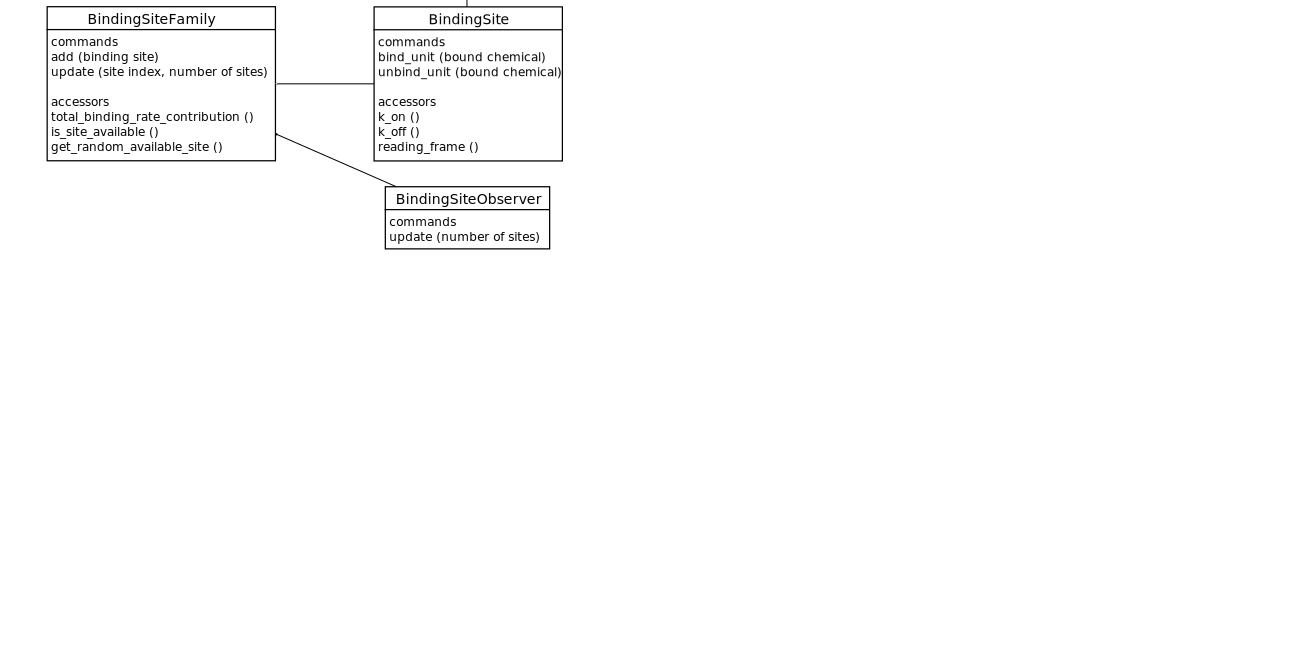
\includegraphics[width=\linewidth]{bindingsitefamily}
  \caption{Schematical view of the Observer pattern used to keep availability of
  binding sites up to date for \texttt{SequenceBinding} reactions.}
\label{fig:det_bsf}
\end{figure}

Every \texttt{BindingSite} is viewed as an \emph{observer} by the \texttt{ChemicalSequence} it belongs to.
Every time a change occurs on the site, the \texttt{BindingSite} is notified.
The latter binding site notifies its \texttt{BindingSiteFamily} using a specific identifier,
letting the family know which binding rate is out of date.
This information is stored in a \texttt{RateValidity} class.
It is only when it is really needed
(\textit{i.e.} when a \texttt{SequenceBinding} wants to access total rate or a random site)
that rates are recomputed.
This avoids useless computations \textit{e.g.} in the case of a translocation,
where a bound unit is first unbound from its \texttt{ChemicalSequence} then rebound.
If the bound unit does not move away from the site, two updates will be sent,
but the rate will only be recomputed once at the end.

% subsection presenting reaction classes
By simple, it is understood that the reaction is performed in one step, instantaneously. The result of a reaction is to change the pools of the reactants and products whenever the reaction happens. {\em When the reaction happens is dealt with in another process}. To describe a reaction, the needed information is thus the pools of the reactants and the enzyme as well as the stoichiometry of the reaction.

\medskip

Let us consider the reaction written in the conventional direction:
$$
  \reactionRev{\underbrace{\sum_{l\in \mathcal{I}_S} m_{l}^SS_{l}}_{Substracts \text{ } S}}{\underbrace{\sum_{l\in\mathcal{I}_P}m_{l}^PP_l}_{Products \text{ } P}}{E}{}.
$$
Note that if this is an enzymatic reaction, then the reaction should not be possible without the enzyme. So that the process is defined by:
\begin{itemize}
  \item inputs:
  \begin{itemize}
    \item the direction of the reaction;
    \item the pool(s) $S_l^{pool}$ of the substract(s);
    \item the pool(s) $E^{pool}$ of the enzyme(s);
    \item the pool(s) $X_l^{pool}$ of the product(s);
  \end{itemize}
  \item parameters: the stoichiometry $m_{l}^S$ and $m_{l}^P$;
  \item processes: if $E^{pool}>0$ (otherwise nothing changes) then change
  \begin{itemize}
    \item if the reaction is in the forward direction: $S_l^{pool} = S_l^{pool} - m_{l}^S$ and $P_l^{pool} = P_l^{pool} + m_{l}^P$;
    \item if the reaction is in the backward direction: $P_l^{pool} = P_l^{pool} - m_{l}^P$ and $S_l^{pool} = S_l^{pool} + m_{l}^S$.
  \end{itemize}
\end{itemize}

\medskip

The above mechanism for process modeling works well as long as every possible 'state' of the reactants are states of the simulator. For instance, we consider the simple reaction (without enzyme for the sake of simplification)
$$
  \reactionIrr{\reactionRev{P_1+P_2}{P_1P_2}{}{}}{Q_1Q_2}{}{}.
$$
In reality, both $P_1$ and $P_2$ have a property, say phosphorized or not. We then have the possible reactions
$$
  \left\{
    \begin{array}{l}
      \reactionIrr{\reactionRev{P_1+P_2}{P_1P_2}{}{}}{Q_1Q_2}{}{} \\
      \reactionIrr{\reactionRev{P_1^*+P_2}{P_1^*P_2}{}{}}{Q_1^*Q_2}{}{} \\
      \reactionIrr{\reactionRev{P_1+P_2^*}{P_1P_2^*}{}{}}{Q_1Q_2^*}{}{} \\
      \reactionIrr{\reactionRev{P_1^*+P_2^*}{P_1^*P_2^*}{}{}}{Q_1^*Q_2^*}{}{} \\
    \end{array}
  \right.
$$
In addition, we can also have the reactions
$$
  \left\{
    \begin{array}{l}
      \reactionRev{P_1 + X}{P_1^*}{}{} \\
      \reactionRev{P_2 + X}{P_2^*}{}{} \\
      \reactionRev{P_1P_2 + X}{P_1^*P_2}{}{} \\
      \reactionRev{P_1P_2 + X}{P_1P_2^*}{}{} \\
      \reactionRev{P_1^*P_2 + X}{P_1^*P_2^*}{}{} \\
      \reactionRev{P_1P_2^* + X}{P_1^*P_2^*}{}{} \\
      \reactionRev{Q_1Q_2 + X}{Q_1^*Q_2}{}{} \\
      \reactionRev{Q_1Q_2 + X}{Q_1Q_2^*}{}{} \\
      \reactionRev{Q_1^*Q_2 + X}{Q_1^*Q_2^*}{}{} \\
      \reactionRev{Q_1Q_2^* + X}{Q_1^*Q_2^*}{}{} \\
    \end{array}
  \right.
$$
Of course, if one puts all the states as described above, the process described above is fine. In this case, the simulator state would be the pools of
$$
  X,\,P_1,\,P_1^*,\,P_2,\,P_2^*,\,P_1P_2,\,P_1^*P_2,\,P_1P_2^*,\,P_1^*P_2^*,\,Q_1Q_2,\,Q_1^*Q_2,\,Q_1Q_2^*,\,Q_1^*Q_2^*
$$
that is 13 states. We want to decrease the number of state. The idea is that the intermediate state are can be computed from the information on $P_1$, $P_1^*$, $P_2$ and $P_2^*$ if we also know the number that are used for these intermediate reactants. Assume, we need the pools of
$$
  X,\,P_1,\,P_1^*,\,P_2,\,P_2^*,\,Q_1Q_2,\,Q_1^*Q_2,\,Q_1Q_2^*,\,Q_1^*Q_2^*.
$$
One would then split in two pools (free and used for $P_1$ and $P_2$ type reactant) the ones of $P_1$, $P_1^*$, $P_2$ and $P_2^*$ leading to also 13 states. Moreover, there is a need for computation to recover the pools of $P_1P_2$, $P_1^*P_2$ , $P_1P_2^*$, and $P_1^*P_2^*$, which is really bad. The relations would have been
$$
  P_{1used}^{pool}+P_{1used}^{*pool} = P_{2used}^{pool}+P_{2used}^{*pool} = (P_1P_2)^{pool}+(P_1^*P_2)^{pool}+(P_1P_2^*)^{pool}+(P_1^*P_2^*)^{pool}
$$
along with
$$
  \left\{
    \begin{array}{l}
      (P_1P_2)^{pool} = \min(P_{1used}^{pool},P_{2used}^{pool}) \\
      (P_1^*P_2^*)^{pool} = \min(P_{1used}^{*pool},P_{2used}^{*pool}) \\
      (P_1^*P_2)^{pool} = P_{2used}^{pool} - (P_1P_2)^{pool} = P_{1used}^{*pool} - (P_1^*P_2^*)^{pool} \\
      (P_1P_2^*)^{pool} = P_{1used}^{pool} - (P_1P_2)^{pool} = P_{2used}^{*pool} - (P_1^*P_2^*)^{pool} \\
    \end{array}
  \right.
$$
Now assume that we only need for the reactant of type $Q_1Q_2$ only the pool of $Q_1Q_2$ separately and that the other pools are not necessary:
$$
  X,\,P_{1free},\,P_{1used},\,P_{1free}^*,\,P_{1used}^*,\,P_{2free},\,P_{2used},\,P_{2free}^*,\,P_{2used}^*,\,Q_1Q_2
$$
We only have 10 states but there is a loss of information as it is now impossible to distinguish between $P_1P_2$ and $Q_1Q_2$ type of reactants. The relation are now
$$
  \left\{
    \begin{array}{l}
      (P_1P_2)^{pool} = \min(P_{1used}^{pool},P_{2used}^{pool}) \\
      (P_1^*P_2^*)^{pool} + (Q_1^*Q_2^*)^{pool} = \min(P_{1used}^{*pool},P_{2used}^{*pool}) \\
      (P_1^*P_2)^{pool} + (Q_1^*Q_2)^{pool} = P_{2used}^{pool} - (P_1P_2)^{pool} = P_{1used}^{*pool} - \min(P_{1used}^{*pool},P_{2used}^{*pool}) \\
      (P_1P_2^*)^{pool} + (Q_1Q_2^*)^{pool} = P_{1used}^{pool} - (P_1P_2)^{pool} = P_{2used}^{*pool} - \min(P_{1used}^{*pool},P_{2used}^{*pool}) \\
    \end{array}
  \right.
$$
Not worth the bother (imagine for 2 properties on $P_1$ and $P_2$ instead of only 1!!!). Use the full information case or limit the number of properties or use the following intermediate solution with the state
$$
  X,\,P_1,\,P_1^*,\,P_2,\,P_2^*,\,Q_1Q_2,\,Q_1^*Q_2,\,Q_1Q_2^*,\,Q_1^*Q_2^*
$$
and with
$$
  (P_1P_2)_{all},\, X_{used}
$$
$(P_1P_2)_{all}$ standing for the whole $P_1P_2,$ $P_1^*P_2$, $P_1P_2^*$ and $P_1^*P_2^*$ and $X_{used}$ standing for $X$ used in $(P_1P_2)_{all}$. A condition for feasibility is then $X_{used}^{pool} \leq 2 (P_1P_2)_{all}^{pool}$. One would have the following possible reactions
$$
  \left\{
    \begin{array}{l}
      \reactionIrr{\reactionRev{P_1+P_2}{(P_1P_2)_{all}}{}{}}{Q_1Q_2}{}{} \\
      \reactionIrr{\reactionRev{P_1^*+P_2}{(P_1P_2)_{all}+X_{used}}{}{}}{Q_1^*Q_2}{}{} \\
      \reactionIrr{\reactionRev{P_1+P_2^*}{(P_1P_2)_{all}+X_{used}}{}{}}{Q_1Q_2^*}{}{} \\
      \reactionIrr{\reactionRev{P_1^*+P_2^*}{(P_1P_2)_{all}+2 X_{used}}{}{}}{Q_1^*Q_2^*}{}{} \\
    \end{array}
  \right.
$$
In addition, we can also have the reactions
$$
  \left\{
    \begin{array}{l}
      \reactionRev{P_1 + X}{P_1^*}{}{} \\
      \reactionRev{P_2 + X}{P_2^*}{}{} \\
      \reactionRev{(P_1P_2)_{all} + X}{(P_1P_2)_{all} + X_{used}}{}{} \\
      \reactionRev{Q_1Q_2 + X}{Q_1^*Q_2}{}{} \\
      \reactionRev{Q_1Q_2 + X}{Q_1Q_2^*}{}{} \\
      \reactionRev{Q_1^*Q_2 + X}{Q_1^*Q_2^*}{}{} \\
      \reactionRev{Q_1Q_2^* + X}{Q_1^*Q_2^*}{}{} \\
    \end{array}
  \right.
$$
The difficulty would be to decide when these reactions can occur. An even 'more' intermediate solution would be to use the states (assuming that $Q_1^*Q_2$ is the reactant of interest since otherwise it is too simple!)
$$
  X,\,P_1,\,P_1^*,\,P_2,\,P_2^*,\,Q_1^*Q_2
$$
and with
$$
  (P_1P_2)_{all},\, X_{Pused},\,(Q_1Q_2)_{all},\, X_{Qused}
$$
with the same constraint as above. The set of reactions are then
$$
  \left\{
    \begin{array}{l}
      \reactionIrr{\reactionRev{P_1+P_2}{(P_1P_2)_{all}}{}{}}{(Q_1Q_2)_{all}}{}{} \\
      \reactionIrr{\reactionRev{P_1^*+P_2}{(P_1P_2)_{all}+X_{Pused}}{}{}}{Q_1^*Q_2}{}{} \\
      \reactionIrr{\reactionRev{P_1+P_2^*}{(P_1P_2)_{all}+X_{Pused}}{}{}}{(Q_1Q_2)_{all}+X_{Qused}}{}{} \\
      \reactionIrr{\reactionRev{P_1^*+P_2^*}{(P_1P_2)_{all}+2 X_{Pused}}{}{}}{(Q_1Q_2)_{all}+X_{Qused}}{}{} \\
    \end{array}
  \right.
$$
In addition, we can also have the reactions
$$
  \left\{
    \begin{array}{l}
      \reactionRev{P_1 + X}{P_1^*}{}{} \\
      \reactionRev{P_2 + X}{P_2^*}{}{} \\
      \reactionRev{(P_1P_2)_{all} + X}{(P_1P_2)_{all} + X_{used}}{}{} \\
      \reactionRev{(Q_1Q_2)_{all} + X}{Q_1^*Q_2}{}{} \\
      \reactionRev{(Q_1Q_2)_{all} + X_{Qused}}{Q_1^*Q_2 + X}{}{} \\
      \reactionRev{(Q_1Q_2)_{all} + X}{(Q_1Q_2)_{all} + X_{Qused}}{}{} \\
    \end{array}
  \right.
$$
Again, the difficulty would be to decide when these reactions can occur.

Finally, it could also be possible to loose even more information by deciding that there only an active form and some non-active forms (one non-active form per type: phosphorized or non-folded -- hum mauvais exemple, pas grave -- for instance). Only the active form can go forward in the pathway; the non-active form must go back into its previous state. Going back to our example with the pathway being:
$$
  \reactionIrr{\reactionRev{P_1+P_2}{P_1P_2}{}{}}{Q_1Q_2}{}{} .
$$
One would consider with this pathway the non-active forms phosphorized and non-folded:
$$
  \left\{
    \begin{array}{l}
      \reactionRev{P_1^{nonFold}}{P_1}{C_1}{} \\
      \reactionRev{P_2^{nonFold}}{P_2}{C_2}{} \\
      \reactionRev{P_1 + X}{P_1^{phosphorized}}{}{} \\
      \reactionRev{P_2 + X}{P_2^{phosphorized}}{}{} \\
      \reactionRev{(P_1P_2)^{nonFold}}{P_1P_2}{C}{} \\
      \reactionRev{P_1P_2 + X}{(P_1P_2)^{phosphorized}}{}{} \\
    \end{array}
  \right.
$$



\medskip

\textcolor[rgb]{1.00,0.00,0.00}{Would be able to model assembly of 30S, 50S and tRNA charging (hum...) if each pool is correctly encoded somewhere as a state.
} 

\subsection{Switches}

\paragraph{Input format}
\begin{verbatim}
Switch <name> <input_bound_chemical> <output_bound_chemical>
SwitchSite <chemical_sequence> <position> <switch_name>
\end{verbatim}

\texttt{Switch}es are intrinsically linked to \texttt{BoundChemical}s
but apply to specific \texttt{BoundUnit}s through \texttt{SwitchSite}s
located on \texttt{ChemicalSequence}s.
Every time an instance of \texttt{input\_bound\_chemical} steps on a switch site,
it \emph{immediately} becomes an \texttt{output\_bound\_chemical}.

For example, during transcription, an RNA polymerase (RNAP) goes through an
initiation state, then loops through several elongation states
(loading of a nucleotide and translocation).
Once it reaches a termination site represented by a \texttt{SwitchSite},
the RNAP leaves its current elongation state and enters termination state.
It stops performing polymerization reactions and typically releases the polymerization product
and unbinds from DNA.\@

A \texttt{Switch} is not considered a reaction because there is no rate associated with it
(switches are performed automatically before the solver chooses the next reaction).
We dedicate a section to these elements because they play a central role in the simulator's philosophy.
The user can use generic reactions that apply in general
(\textit{e.g.} transcription of any gene based on its sequence)
and use switches every time something more specific is needed.
As seen before, termination sites for transcription are expected to be \textit{SwitchSite}s.
Similarly, important regulation sites can be implemented using \textit{SwitchSite}s.

% subsection presenting solver related classes

\subsection{Solver loop}

\subsubsection{Solver class}

\subsection{Events}

\texttt{Event}s enable users to change molecule numbers outside of the solver loop
at specific times~\reffigp{fig:events}.
A \texttt{Simulation} instance handles both a \texttt{Solver} instance and
an \texttt{EventHandler} instance.
Every time an event timing is reached, the solver loop is stopped,
the event(s) is (are) performed, the solver is reinitialized and the simulation resumes.
Different \texttt{Event} implementations are offered to modify molecule numbers in a convenient way.

\begin{figure}[!h]
  \centering
  \includegraphics[width=\linewidth]{events}
  \caption{
  \texttt{Event}s: another way to modify chemical concentrations aside from reactions,
  \textit{e.g.} to simulate the injection of a chemical inside a cell.
  }
\label{fig:events}
\end{figure}

% subsection presenting input/output related classes
\subsection{Events}

\texttt{Event}s enable users to change molecule numbers outside of the solver loop at specific times~\reffigp{fig:events}. A \texttt{Simulation} instance handles both a \texttt{Solver} instance and an \texttt{EventHandler} instance. Every time an event timing is reached, the solver loop is stopped, the event(s) is (are) performed, the solver is reinitialized and the simulation resumes. Different \texttt{Event} implementations are offered to modify molecule numbers in a convenient way.

\begin{figure}[!h]
  \centering
  \includegraphics[width=\linewidth]{events}
  \caption{\texttt{Event}s: another way to modify chemical concentrations aside from reactions, \textit{e.g.} to simulate the injection of a chemical inside a cell.}
  \label{fig:events}
\end{figure}

\subsection{Input/Output handling}

\subsubsection{Simulator Input}

The simulator needs the following to work:
\begin{itemize}
  \item A general input file defining simulation parameters. A sample file is provided were all options are described (\textit{e.g.} length of simulation, what to output, algorithm variants). One important parameter is the location of the files the simulator should open to read reactants, reactions and events.
  \item An arbitrary number of files where reactants, reactions and events are declared. The simulator solves dependencies across files, it is not necessary to declare reactants in the same file as or before reactions using them.
\end{itemize}

Caution:
\begin{itemize}
\item All reactants must be declared in some file with their appropriate type (\textit{e.g.} \texttt{FreeChemical} or \texttt{BoundChemical}).
\item Multiple declarations are forbidden, a name cannot be reused.
\end{itemize}

\subsubsection{Simulator Output}

Outputs provided by the simulator are:
\begin{itemize}
\item A general output file logging parametes used for simulation (input files used, random seed, algorithms used, etc.).
\item A concentration file with the number of molecules over time (for the chemicals and at a time step defined in the parameter file).
\item If a \texttt{DoubleStrand} was added in the chemicals to ouput, a replication file describing replication advancement of that \texttt{DoubleStrand}.
\end{itemize}

